\documentclass{anstrans}
%%%%%%%%%%%%%%%%%%%%%%%%%%%%%%%%%%%
\title{Modeling potential JCPOA diversion scenarios with Cyclus}
\author{Baptiste Mouginot,$^{*}$ Kathryn Mummah,$^{*}$ Paul P.H. Wilson$^{*}$}

\institute{
$^{*}$University of Wisconsin-Madison, WI
}

\email{mouginot@wisc.edu \and mummah@wisc.edu \and paul.wilson@wisc.edu}

% Optional disclaimer: remove this command to hide
% \disclaimer{Notice: this manuscript is a work of fiction. Any resemblance to
% actual articles, living or dead, is purely coincidental.}

%%%% packages and definitions (optional)
\usepackage{graphicx} % allows inclusion of graphics
\usepackage{booktabs} % nice rules (thick lines) for tables
\usepackage{microtype} % improves typography for PDF
\usepackage{float}

\newcommand{\SN}{S$_N$}
\renewcommand{\vec}[1]{\bm{#1}} %vector is bold italic
\newcommand{\vd}{\bm{\cdot}} % slightly bold vector dot
\newcommand{\grad}{\vec{\nabla}} % gradient
\newcommand{\ud}{\mathop{}\!\mathrm{d}} % upright derivative symbol

\begin{document}
%%%%%%%%%%%%%%%%%%%%%%%%%%%%%%%%%%%%%%%%%%%%%%%%%%%%%%%%%%%%%%%%%%%%%%%%%%%%%%%%
\section{Introduction}



\section{Cascade Enrich Construction}
\subsection{Centrifuge properties}




\subsection{Explored Cases}





%%%%%%%%%%%%%%%%%%%%%%%%%%%%%%%%%%%%%%%%%%%%%%%%%%%%%%%%%%%%%%%%%%%%%%%%%%%%%%%%
%% \appendix
%% \section{Appendix}
%%
%% Numbering in the appendix is different:
%% \begin{equation} \label{eq:appendix}
%%   2 + 2 = 5\,.
%% \end{equation}
%% and another equation:
%% \begin{equation} \label{eq:appendix2}
%%   a + b = c\,.
%% \end{equation}
%%
%%%%%%%%%%%%%%%%%%%%%%%%%%%%%%%%%%%%%%%%%%%%%%%%%%%%%%%%%%%%%%%%%%%%%%%%%%%%%%%%
%% \section{Nomenclature}
%%
%% \begin{table}[H]
%%     \centering
%%     \begin{tabular}{l|l}
%% %         &  \\
%%         $N$ & Feed assay \\
%%         $N'$ & Product assay \\
%%         $N''$ & Tails assay \\
%%         $\alpha$ & Feed to product enrichment factor \\
%%         $\beta$ & Feed to tail enrichment factor \\
%%         $\theta$ & Cut
%%     \end{tabular}
%% %    \caption{Caption}
%%     \label{tab:my_label}
%% \end{table}

%% \begin{figure}[ht] % replace 't' with 'b' to force it to be on the bottom
%%   \centering
%%   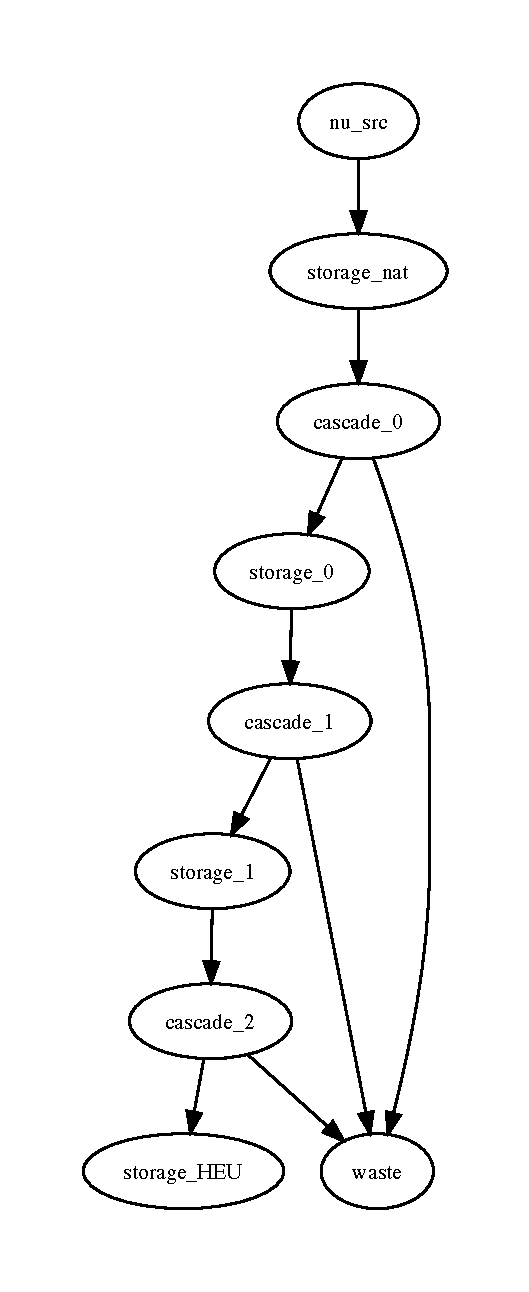
\includegraphics[scale=0.68]{flow_case_2_no_recy.pdf}
%%   \caption{Illustration of the material flow between the different level of
%%       cascades without tail recycling, in this diagram, nu\_src corresponds to
%%       an infinite source of natural uranium, cascade\_ $\{n\}$ and storage\_
%%       $\{n\}$ to the cascade and the storage getting the products of the
%%       cascades at the level $\{n\}$.}\label{fig:flow}
%% \end{figure}

%% \begin{table}[htb]
%% \centering
%%   \caption{Summary of cascade properties for each level.}
%% \begin{tabular}{cllll}
%% \toprule
%% 
%% Level   &           & Assay     &       & Machines  \\
%%         & Feed      & Product   & Feed  &           \\
%% \midrule
%% 0       & 0.0071    & 0.0413    & 0.0029 & 167       \\
%% 1       & 0.0413    & 0.2043    & 0.0173 & 169       \\
%% 2       & 0.2043    & 0.5941    & 0.0971 & 168       \\
%% 3       & 0.5941    & 0.8834    & 0.3915 & 168       \\
%% 4       & 0.8834    & 0.9735    & 0.7746 & 169       \\
%% 
%% \bottomrule
%% \end{tabular}
%% 
%%   \label{tab:cascadelvl}
%% \end{table}

%%%%%%%%%%%%%%%%%%%%%%%%%%%%%%%%%%%%%%%%%%%%%%%%%%%%%%%%%%%%%%%%%%%%%%%%%%%%%%%%
\section{Acknowledgments}
This work was funded by the Consortium for Verification Technology under
Department of Energy National Nuclear Security Administration award number
DE-NA0002534

%%%%%%%%%%%%%%%%%%%%%%%%%%%%%%%%%%%%%%%%%%%%%%%%%%%%%%%%%%%%%%%%%%%%%%%%%%%%%%%%
\bibliographystyle{ans}
\bibliography{bibliography}
\end{document}
